\chapter{Problem Analysis} \label{chap:problemanalyse}

The problem analysis for this project begins with the chosen question from the 2020 project catalogue for Software at Aalborg University. The group decided on the first question regarding simulation of COVID-19. The full project description can be found in Appendix \vref{P1Katalog}.

\section{Introducing the Problem Analysis}
To define our problem, we made a mindmap of questions to figure out geographical location (where?), interested parties (who?), time frame (when?) and so on. The analytical model is shown in figure \ref{fig:HV-mindmap}.

\begin{figure}[H]
    \centering
    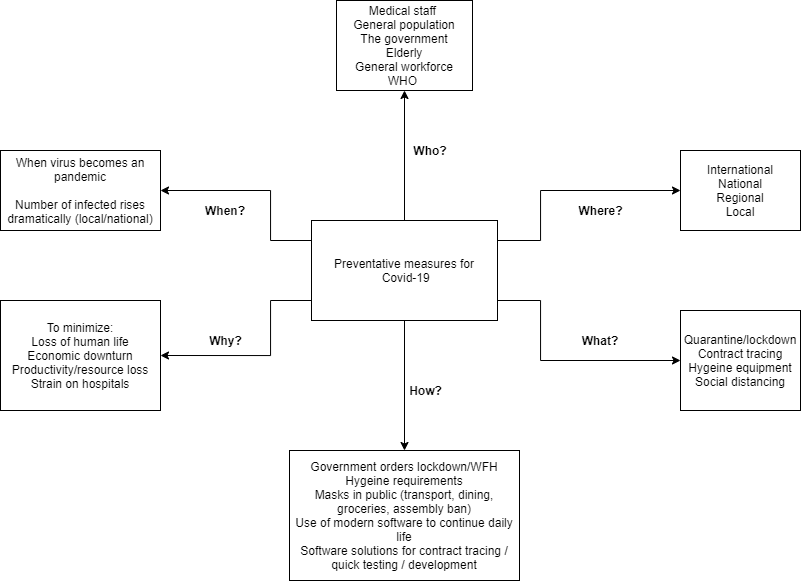
\includegraphics[width=0.75\textwidth]{0_billeder/HV-Mindmap.png}
    \caption{Mindmap of questions or, in Danish, HV-mindmap.}
    \label{fig:HV-mindmap}
\end{figure}

It was decided to continue with the questions raised regarding "how" and "why", as these branches on the mindmap aid the focus on simulation that is imperative to the project.

Our goal is to make a simulation of COVID-19 spread as well as the effects of preventive measures, namely contact tracing. Throughout our theoretical outlining, we wish to focus on software solutions that predict the spread (and how one might limit the spread) of COVID-19. Specifically, our goal is to centre our work around contact tracing as a variable as well as researching other meaningful variables that can prevent further spread of COVID-19.

Before formulating a concise problem statement, some theoretical foundation about COVID-19 is naturally needed. Therefore, the following describes several key aspects of COVID-19, such as the basic virology of the illness, SARS-CoV-2, societal factors that can influence the spread as well as several preventive measures - including contact tracing - of COVID-19.